\chapter{Conclusions}
\label{ch:conslucions}

\section{Summary}

A brute-force approach was used to classify bruxism-related events. Four traditional classifiers were combined with different recorded time-series sets. Quaternion data from the IMUs placed on the back sides of the jaw with the random forest classifier yielded the best performance score with the least amount of sensors. It achieved 88\% accuracy. The best performing score overall was 91.5\% achieved by the random forest classifier with the BNO055 gyroscope and quaternion, eSense earables accelerometer, masseter, and temporalis time-series (from both sides each). As the IMUs tend to be cheaper than the EMG and are already present in various wearables (e.g. eSense earables) it once more confirms their potential in bruxism detection.

This study summarizes the use of 5 different devices with the scope of classifying bruxism-related events. The COVID-19 Pandemic may have also started another wave of a bruxism pandemic. The overall increase in the stress level may as well increase the prevalence of awake bruxism. A cheap and practical device is needed, that will have the ability to diagnose potential patients before it will lead to discomfort or teeth damage. The device selection was done based on previous research in the field and then combined together in a custom-built prototype. While selecting the devices we tried to maximize the use of the \emph{potential area} on the human head and neck, where a bruxism-induced signal may be recorded. A user study was designed to include bruxism-related jaw movements (clenching, grinding, and sliding) and contrasting \emph{regular} jaw movements (talking, drinking, chewing, smiling, etc.). All of the selected devices for the prototype were used at the same time during every user study.

\section{Limitations \& Future Work}

The study was done in a controlled environment, and the presented results may only be compared only in the context of this study. It is important to mention, that the custom-built prototype was just used as a framework to generate a reference.

The results of this study show that the sensor fusion of the IMU data appears the most promising feature to have a wearable device in the vicinity of the jaw. The closer to the jaw, the better the accuracy.

Bruxism happens mostly unconsciously. Prolonged periods appear during a patient's sleep. An EMG-oriented device may actually be a better choice for a sleep use case. A comparison with a much more mature device with IMUs is needed to be done in-the-wild.

Alternative ways of labeling and data segmentation can be explored. In an in-the-wild environment, bigger duration trends can be tracked. The performance in such cases should ideally correlate with the lessening of the bruxism occurrence over time.

More advanced machine learning approaches for time-series classification may also be useful.

The labeling of the data was in itself a very cumbersome and error-prone process. As we had to rely on visual clues in the time-series, as well as on timing (estimated duration of performed tasks and the duration of the pauses in-between). The keyboard event listener coroutine (see ch. \ref{ch:Implementation}) can be improved and extended to create the labels during the runtime. Either the experimenter or the participant itself can press (or hold) a button, to indicate a start or end of an action. This coroutine can be completely extracted from the framework and used as a separate device or as a software module.

\section{Challenges}
\label{sub:attachment_problems}

\subsection{eSense earables}
\label{par:esense_attachment}

Because of the design of the earables to be placed in the ear, some of the participants had trouble fitting them inside of their ears. Because the audio playback or audio recording with the built-in microphone was out of the scope of this study, the earables were secured with skin-friendly tape.

\subsection{EMG-Electrodes}
\label{par:emg_attachment}

To collect EMG signals, special electrodes must be placed on the skin surface covering the target muscle. It is not a trivial task, as the anatomy of the participant dictates the optimal spot of the electrode placement. The following research paper was used as a reference to find the optimal EMG spots \cite{sabaneeff2017proposal}.

\begin{figure}[h!]
\centering
 \begin{subfigure}[b]{0.49\textwidth}
    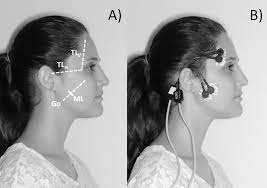
\includegraphics[width=\textwidth]{src/media/study/emg1.jpeg}
    \caption{ (A) Reference lines drawn on the face of a volunteer;
(B) electrodes positioned over the AT and SM muscles. \cite{sabaneeff2017proposal}}
  \end{subfigure}
 \hfill
 \begin{subfigure}[b]{0.49\textwidth}
    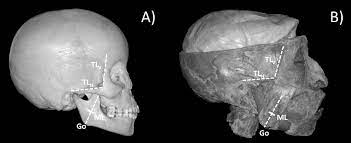
\includegraphics[width=\textwidth]{src/media/study/emg2.jpeg}
    \caption{ (A) The lateral view of the skull shows the reference lines used
in this study: TLV, TLH, and ML. The small thick line represents an
intersection at 40\% the length of ML from Go landmark; (B) Lateral
view of deep facial planes, evidencing the AT and SM muscles and their
relationship with anatomical landmarks and reference lines adopted. \cite{sabaneeff2017proposal}}
  \end{subfigure}
\caption{Optimal EMG spots for masticatory muscles by \cite{sabaneeff2017proposal}}
\label{image:real-emg}
\end{figure}

The following EMG electrode fig. \ref{image:emg_electrode} was used. For every target muscle, a pair of such electrodes is needed. Additionally, a reference electrode must be also placed on a neutral part of the head. The reference cables were fused together and connected to an electrode placed under the participant's chin.

The masticatory muscles are relatively small, so a slice of the adhesive foam was removed to bring the conductive parts of the two electrodes placed on one muscle, closer together. Even with this modification, the temporalis muscle was hard to capture, as even a misplace of 1mm from the optimal spot will introduce noise, or will capture the EMG signal of the nearby muscles (i.e. orbicularis muscle responsible for blinking).

\begin{figure}[h]
\centering
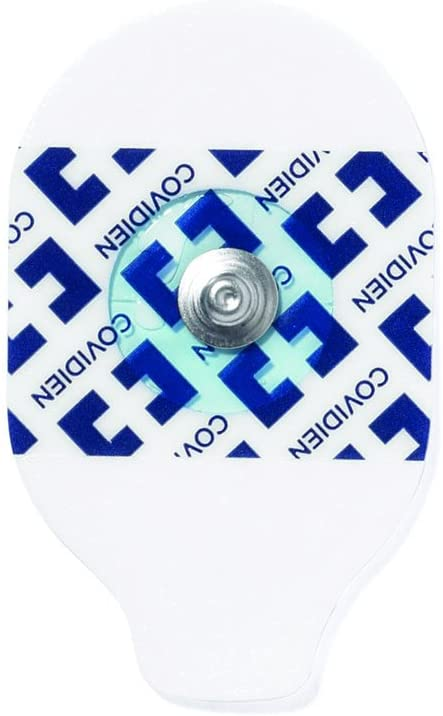
\includegraphics[width=0.2\textwidth]{src/media/study/electrode.jpg}
\caption{EMG electrode (57 x 34mm)}
\label{image:emg_electrode}
\end{figure}

\subsection{Throat Microphone}
\label{par:mic_attachment}

The throat microphone used in this study didn't have any adjustment possibilities. 2 of the participants had a smaller neck circumference, and as a result, it was not possible to capture the eventual vibrations that would propagate through the neck.

